\section{Assumption and Terminology}
\label{sec:assumption}

We assume that the Compute Unified Device Architecture (CUDA) is used
for GPU programming~\cite{NVIDIA_CUDA}.
A unit of code that is individually launched on the GPU is called
a \textit{kernel}.
The kernel is composed of multiple \textit{threads} that execute the
code in parallel.
A unit of threads that are co-scheduled by hardware is called a
\textit{block}, while a collection of blocks for the corresponding
kernel is called a \textit{grid}.  
The maximum number of threads that can be contained by an individual
block is defined by the GPU architecture.

CUDA uses a set of an application programming interface (API) functions
to manage the GPU.
A typical CUDA program takes the following steps: (i) allocate space
to the device memory, (ii) copy input data to the allocated device memory
space, (iii) launch the program on the GPU, (iv) copy output data back
to the host memory, and (v) free the allocated device memory space. 
The scope of this paper is related to (ii) and (iv).
Particularly we use the \texttt{cuMemCopyHtoD()} and the
\texttt{cuMemCopyDtoH()} functions provided by the CUDA Driver API,
which correspond to (ii) and (iv) respectively.
Since an open-source implementation of these functions is
available~\cite{Kato_ATC12}, we modify them to accommodate various data
transfer methods investigated in this paper.
While they are synchronous data transfer functions, CUDA also provides
asynchronous data transfer functions.
In this paper, we restrict our attention to the synchronous data
transfer functions for simplicity of description, but partly similar
performance characteristics can also be applied for the asynchronous
ones.

In order to focus on the performance of data transfers between the host
and the device memory, we allocate a data buffer to the pinned host
memory rather than the typical heap allocated by \texttt{malloc()}.
This pinned host memory space is mapped to the PCIe address and is never
swapped out.
It is also accessible to the GPU directly.

Our computing platform contains a single set of the CPU and the GPU.
Although we restrict our attention to CUDA and the GPU, the notion of
the investigated data transfer methods is well applicable to other
heterogeneous compute devices.
GPUs are currently well-recognized forms of the heterogeneous compute
devices, but emerging alternatives include the Intel Many Integrated
Core (MIC) and the AMD Fusion technology.
The programming models of these different platforms are almost identical
in that the CPU controls the compute devices.
Our future work includes an integrated investigation of these different
platforms.

\begin{figure}[!t]
 \centering
 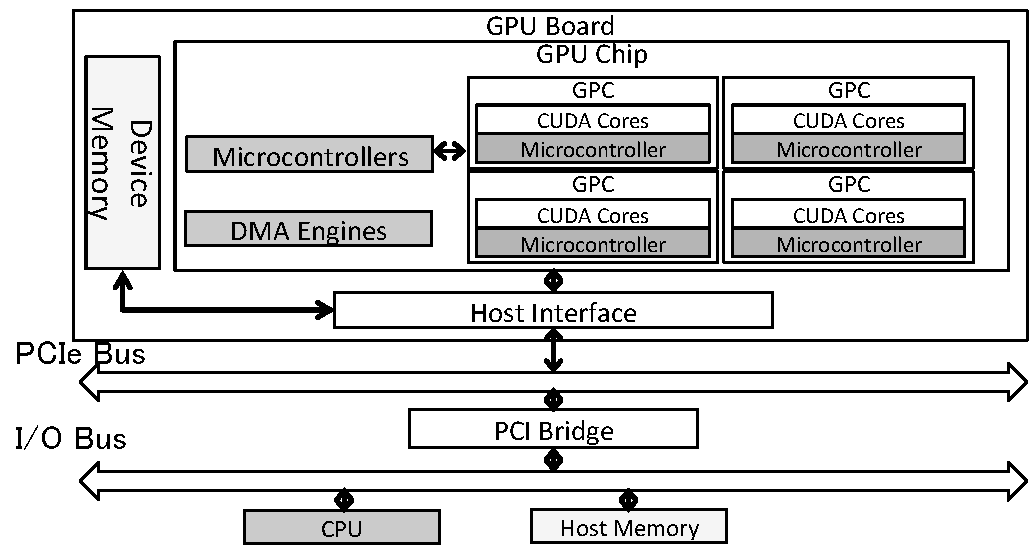
\includegraphics[width=0.49\textwidth]{figure/Method/pci_gpu.pdf}
 \caption{Block diagram of the target system.}
 \label{fig:pci_gpu}
\end{figure}

Figure~\ref{fig:pci_gpu} shows a summarized block diagram of the target
system.
The host computer consists of the CPU and the host memory communicating
on the system I/O bus.
They are connected to the PCIe bus to which the GPU board is also
connected.
This means that the GPU is visible to the CPU as a PCIe device.
The GPU is a complex compute device integrating a lot of hardware
functional units on a chip.
This paper is only focused on the CUDA-related units.
There are the device memory and the GPU chip connected through a high
bandwidth memory bus.
The GPU chip contains graphics processing clusters (GPCs), each of which
integrates hundreds of processing cores, \textit{a.k.a}, CUDA cores.
The number of GPCs and CUDA cores is architecture-specific.
For example, GPUs based on the NVIDIA GeForce Fermi
architecture~\cite{NVIDIA_Fermi} used in this paper support at most 4
GPCs and 512 CUDA cores.
Each GPC is configured by an on-chip microcontroller.
This microcontroller is wimpy but is capable of executing firmware code
with its own instruction set.
There is also a special \textit{hub} microcontroller, which broadcasts the
operations on all the GPC-dedicated microcontrollers.
In addition to hardware DMA engines, this paper investigates how these
detailed hardware components operate and interact with each other to
support data transfers in GPU computing.

It should be noted that our target system is not limited to a specific
GPU but can be applied for most other GPUs and heterogeneous compute
devices connected upon the PCIe bus, though each detailed specification
may be different depending on their architectures.
Concretely PCIe compute devices are typically visible to the CPU through
the memory-mapped I/O space over some PCI base address register (BAR)
and they often equip on-chip microcontrollers to run some firmware
code.